\section{Einleitung}
\subsection{Einführung in die Thematik}
\blindtext\nomenclature{W3C}{World Wide Web Consortium}
\blindtext\footcite[][]{mswpf}

\subsection{Problemstellung und Zielsetzung}
\blindtext

\subsection{Methodischer Aufbau der Arbeit}
\blindtext

\section{Hauptteil}
\subsection{Grundlagen der Wirtschaftsinformatik}
\blindtext\footcite[][]{msdatabind}\footcite[][]{Atypisch}\footcite[][34]{Digitaloekonomie}
\blindenumerate
\Blindtext\footcite[][415-426]{Tanenbaum2016}

\begin{figure}[!htb]
    \caption{Terminal}
    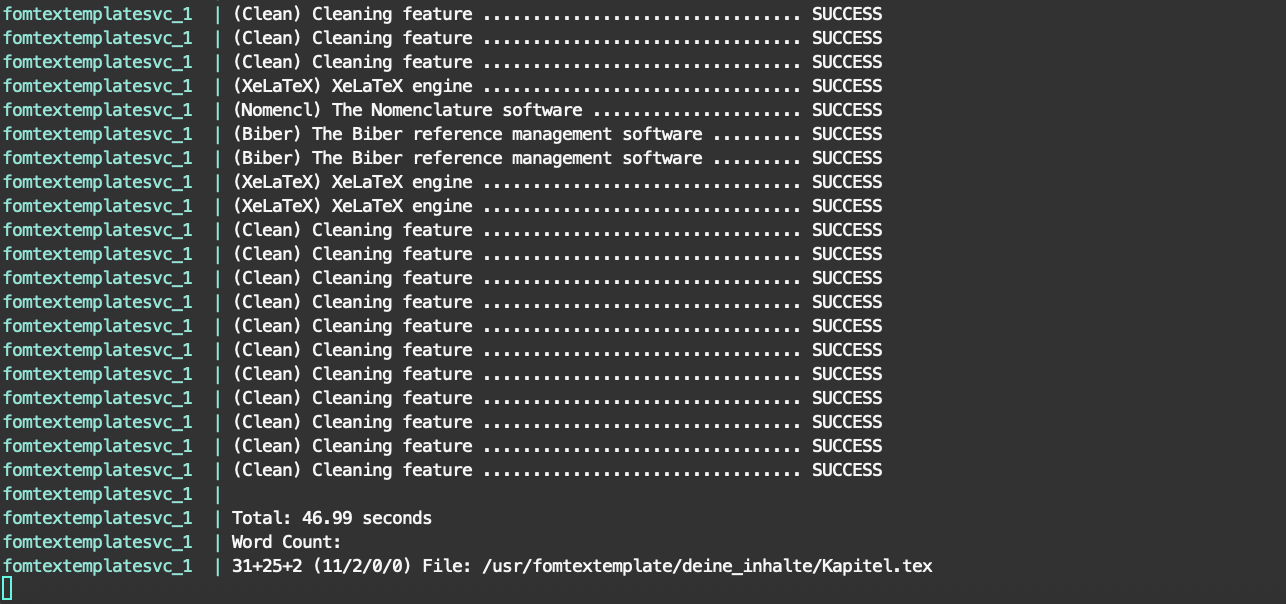
\includegraphics[width=1\textwidth]{.github/terminal}
    \captionsetup{width=1\textwidth}
    \capquelle{\cite[][200]{bsp}}\label{abb_bsp}
\end{figure}
\blindtext

\subsubsection{Design-Prinzip der Separierung von Verantwortlichkeiten}
\blindtext\footcite[][79]{Schelinski2019}

\begin{table}[h]
    \centering
    \begin{threeparttable}
        \centering
        \caption{Tabelle}
        \begin{tabular}{cccccccc}
            {$m$} & {$\Re\{\underline{\mathfrak{X}}(m)\}$} & {$-\Im\{\underline{\mathfrak{X}}(m)\}$} & {$\mathfrak{X}(m)$} & {$\frac{\mathfrak{X}(m)}{23}$} & {$A_m$} & {$\varphi(m)\ /\ ^{\circ}$} & {$\varphi_m\ /\ ^{\circ}$} \\
            \hline
            1  & 16.128 & +8.872 & 16.128 & 1.402 & 1.373 & -146.6 & -137.6 \\
            2  & 3.442  & -2.509 & 3.442  & 0.299 & 0.343 & 133.2  & 152.4  \\
            3  & 1.826  & -0.363 & 1.826  & 0.159 & 0.119 & 168.5  & -161.1 \\
            4  & 0.993  & -0.429 & 0.993  & 0.086 & 0.08  & 25.6   & 90     \\
            5  & 1.29   & +0.099 & 1.29   & 0.112 & 0.097 & -175.6 & -114.7 \\
            6  & 0.483  & -0.183 & 0.483  & 0.042 & 0.063 & 22.3   & 122.5  \\
            7  & 0.766  & -0.475 & 0.766  & 0.067 & 0.039 & 141.6  & -122   \\
            8  & 0.624  & +0.365 & 0.624  & 0.054 & 0.04  & -35.7  & 90     \\
            9  & 0.641  & -0.466 & 0.641  & 0.056 & 0.045 & 133.3  & -106.3 \\
            10 & 0.45   & +0.421 & 0.45   & 0.039 & 0.034 & -69.4  & 110.9  \\
            11 & 0.598  & -0.597 & 0.598  & 0.052 & 0.025 & 92.3   & -109.3 \\
            \hline
        \end{tabular}
        \begin{tablenotes}[flushleft]
        \item \normalsize{Quelle: \cite[][200]{bsp}}
        \end{tablenotes}
    \end{threeparttable}
\end{table}

\Blindtext\footcite[][34]{Digitaloekonomie}
\blinditemize
\blindtext\footcite[][511]{Tanenbaum2016}

\subsubsection{LaTeX-Befehle}
    \textnormal{Normale Schrift} 
    \textbullet\addspace \textbf{fette Schrift} 
    \textbullet\addspace \textit{kursive Schrift} 
    \textbullet\addspace \textsl{schiefe Schrift} 
    \textbullet\addspace \underline{unterstrichen} 
    \textbullet\addspace \texttt{Schreib\-ma\-schi\-ne} 
    \textbullet\addspace \textsf{Sans Serif} 
    \textbullet\addspace \textrm{Roman} 

\subsection{Test: Silbentrennung - Gegenüberstellung darf nicht in den weißen Rand laufen}
Im zweiten Kapitel wird zunächst der Begriff \textit{Bring Your Own Device} (BYOD) definiert. Darauffolgend wird dargelegt welche Fokusse gesetzt werden sollen und Schlussfolgerungen gezogen, sowie eine Sicherheitsrichtlinie abgeleitet. Welche als Grundlage einer Gegenüberstellung mit etablierten Konzepten dient, sodass Strategien erörtert werden können. 

\section{Schluss}
\subsection{Fazit}
\blindtext (vgl. Abbildung \ref{abb_bsp}).

\subsection{Ausblick}
\blindtext
